\section{Algoritmen}
\subsection{Algemene uitleg}
De manier van aanpak werd dus veranderd. In plaats van een border langsheen de rand van het scherm te creëren is geopteerd geweest om de diagonalen te verbinden (een groene en een blauwe) en op het snijpunt wordt een lichtblauwe bol weergegeven, zie figuur \ref{fig:screen}. Door deze aanpassing wordt het makkelijker om te achterhalen tot welk island een los deel van een scherm behoort. De huidige voorwaarden om een scherm te kunnen detecteren zijn dat twee aanliggende hoeken en het middelpunt zichtbaar moeten zijn. Achter het kruis wordt nog steeds de barcode geplaatst om de schermen te identificeren.
Een offset werd toegevoegd tijdens het vormen van de islands omdat zo de ruis verwijderd wordt rond de overgangen van de achtergrondkleuren.Hieronder volgt een opsomming van de aangepaste methoden die toegepast worden op de invoer afbeelding in chronologische volgorde. Ongewijzigde methoden worden achterwege gelaten in deze opsomming.

\begin{figure} [h]
	\center
	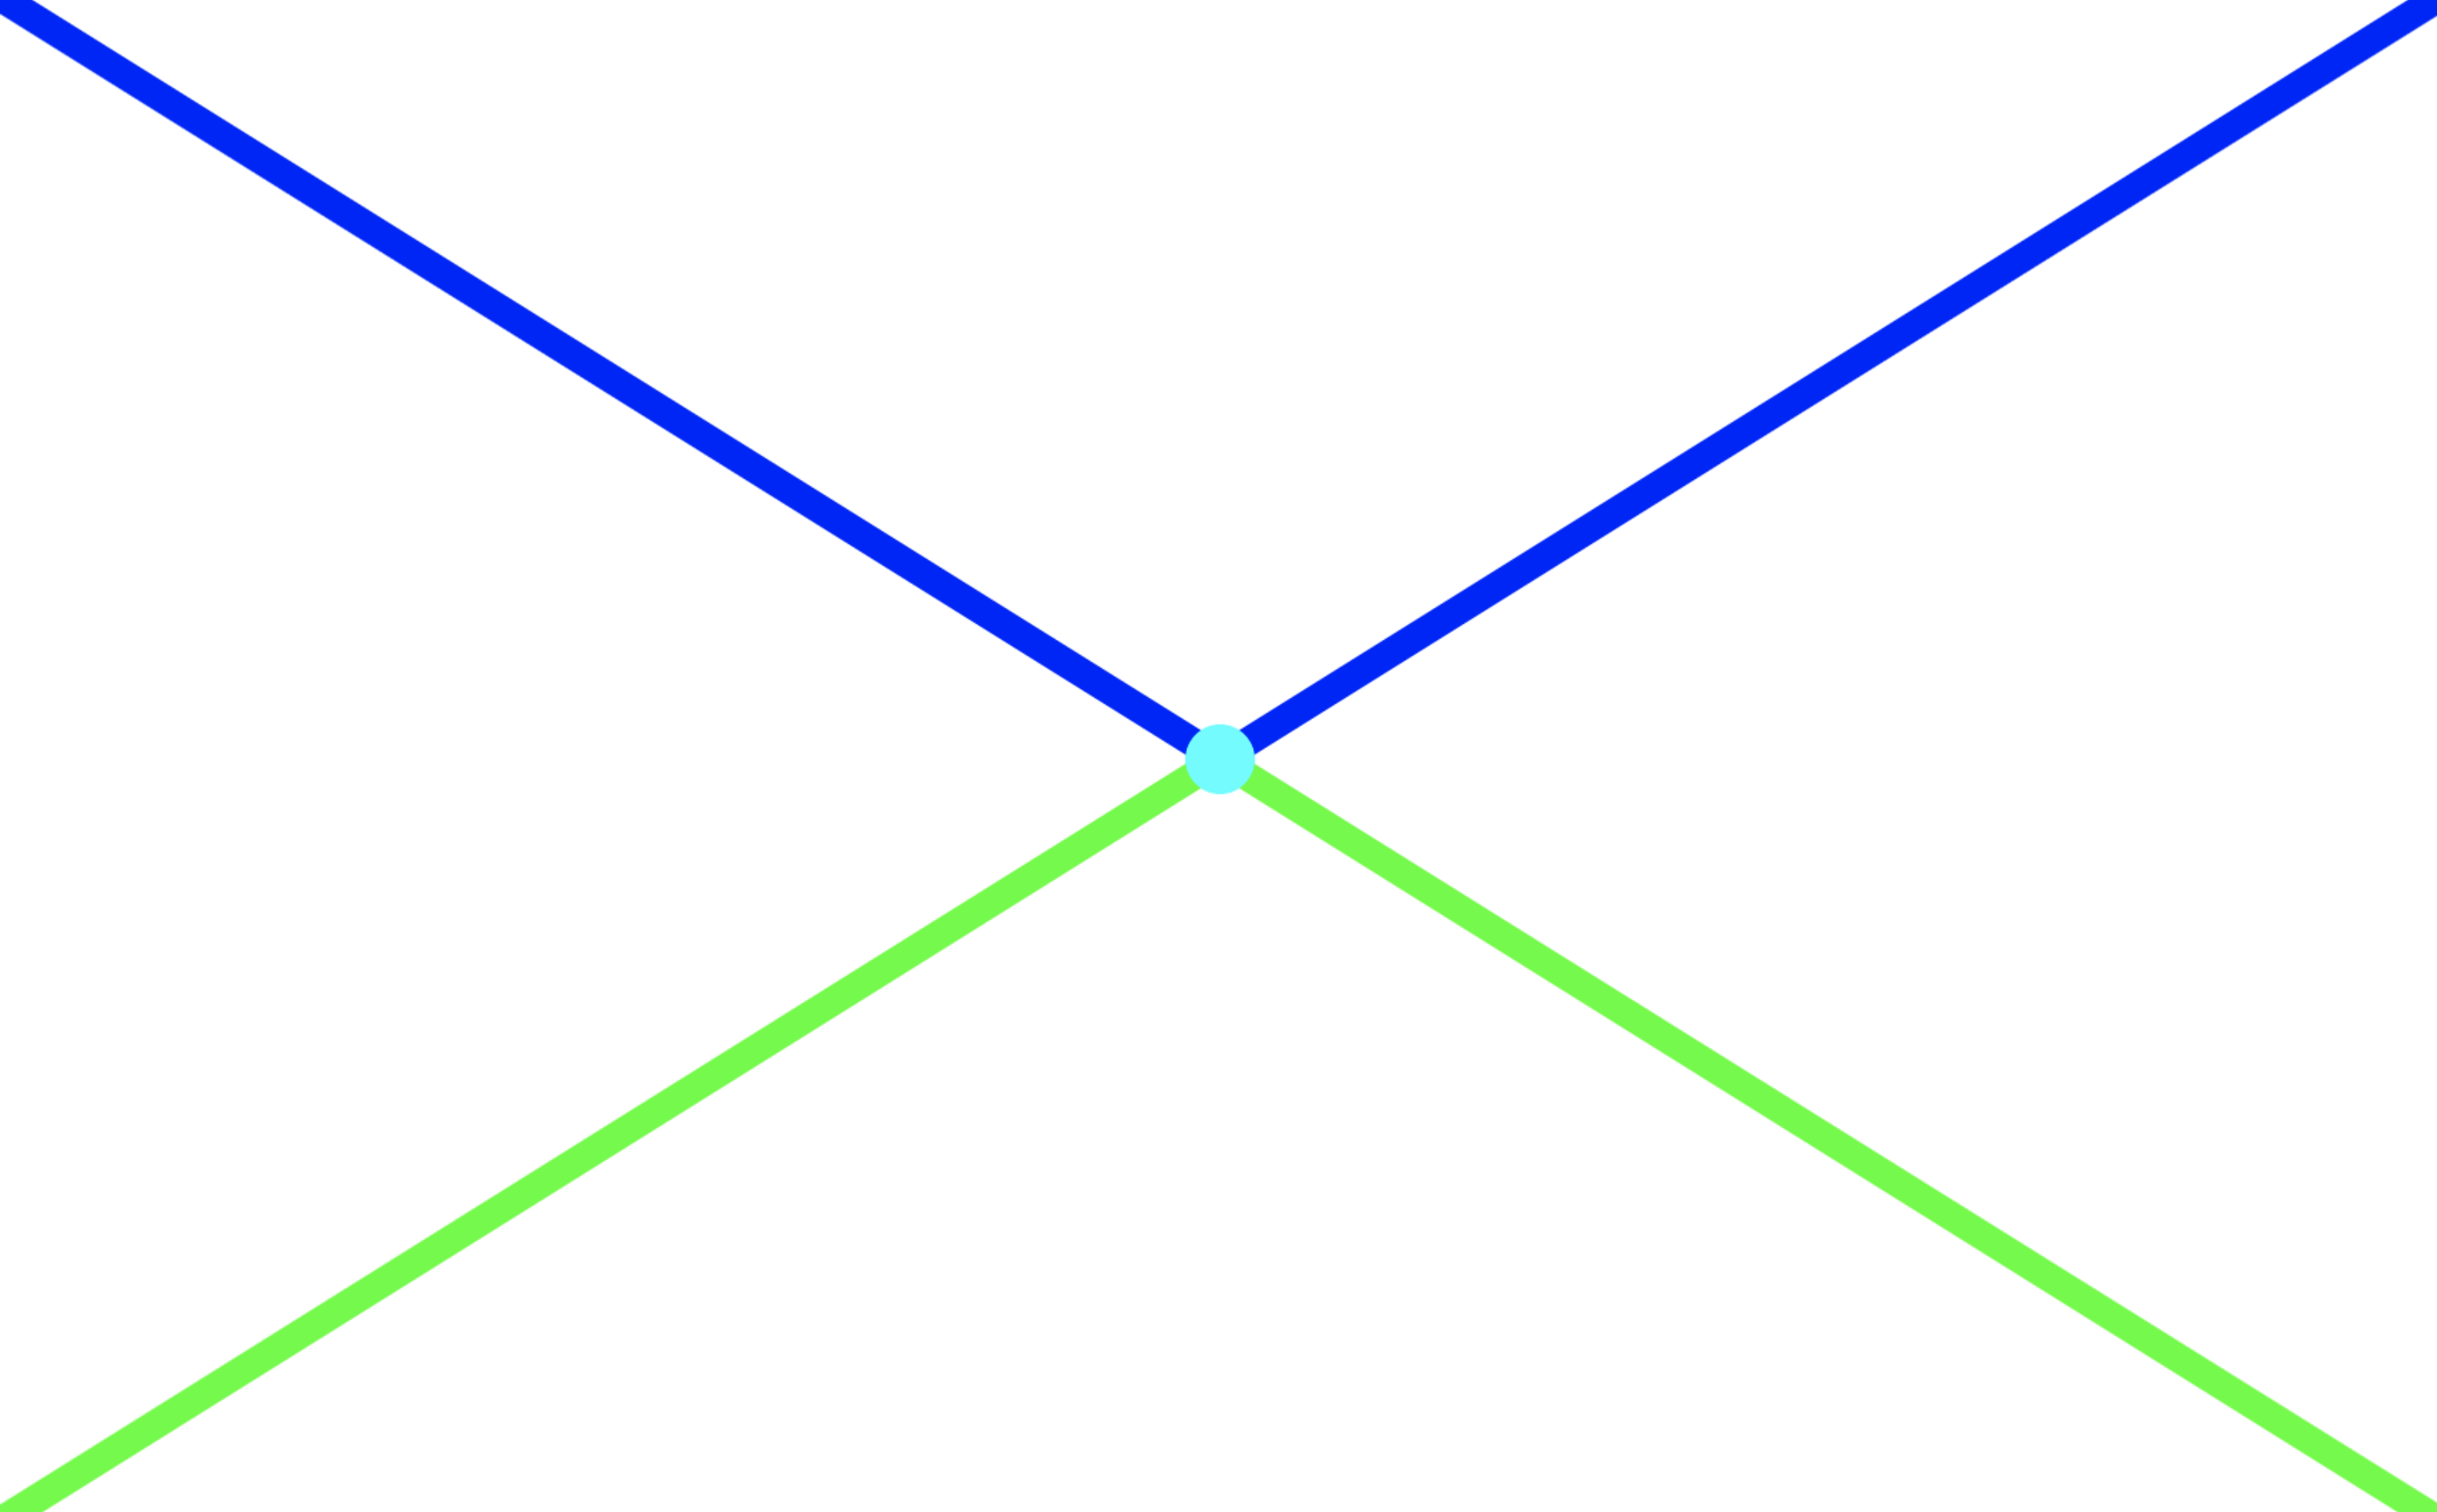
\includegraphics[width=\textwidth]{screen}
	\caption{Nieuwe schermachtergrond}
	\label{fig:screen}
\end{figure}

\subsection{Kleuren masker}
Deze methode werkt nog steeds hetzelfde als bij de vorige taak. Wel werd een extra kleur toegevoegd voor het middelpunt. Groene pixels krijgen een waarde 1, blauwe 2 en lichtblauwe 3 in de matrix. Tijdscomplexiteit van de methode blijft door deze aanpassing onveranderd, nog steeds moeten alle pixels overlopen worden.

\subsection{Find Islands}
De detectie van een scherm start nog steeds met het zoeken van eilanden van pixels die niet zwart zijn. Bij overlap van schermen en dus mogelijks losliggende stukken scherm in onze matrix, wordt het zeer belangrijk om bij te houden tot welke island een niet zwarte pixel wel degelijk hoort. Hiervoor krijgt elke gestarte island een ID (met tussensprongen van vier om nog steeds de kleuren te kunnen onderscheiden in onze matrix). Wanneer tijdens de floodfill dan een pixel gevonden wordt die bij een reeds gestartte island zou moeten horen, wordt de waarde van deze pixel geïncrementeerd met de desbetreffende ID. \cite{floodfill} Bijvoorbeeld stel dat er reeds een island was en er een tweede ontdekt wordt. Dan krijgt deze tweede island een ID met waarde 3. Een groene pixel die dan tot deze island behoort zal waarde 4 hebben. Eens alle pixels gevonden zijn wordt omtrekkend kader opgesteld aan de hand van de minimum en maximum x-- en y--waarden \ref{fig:island}.

\begin{figure} [h]
	\center
	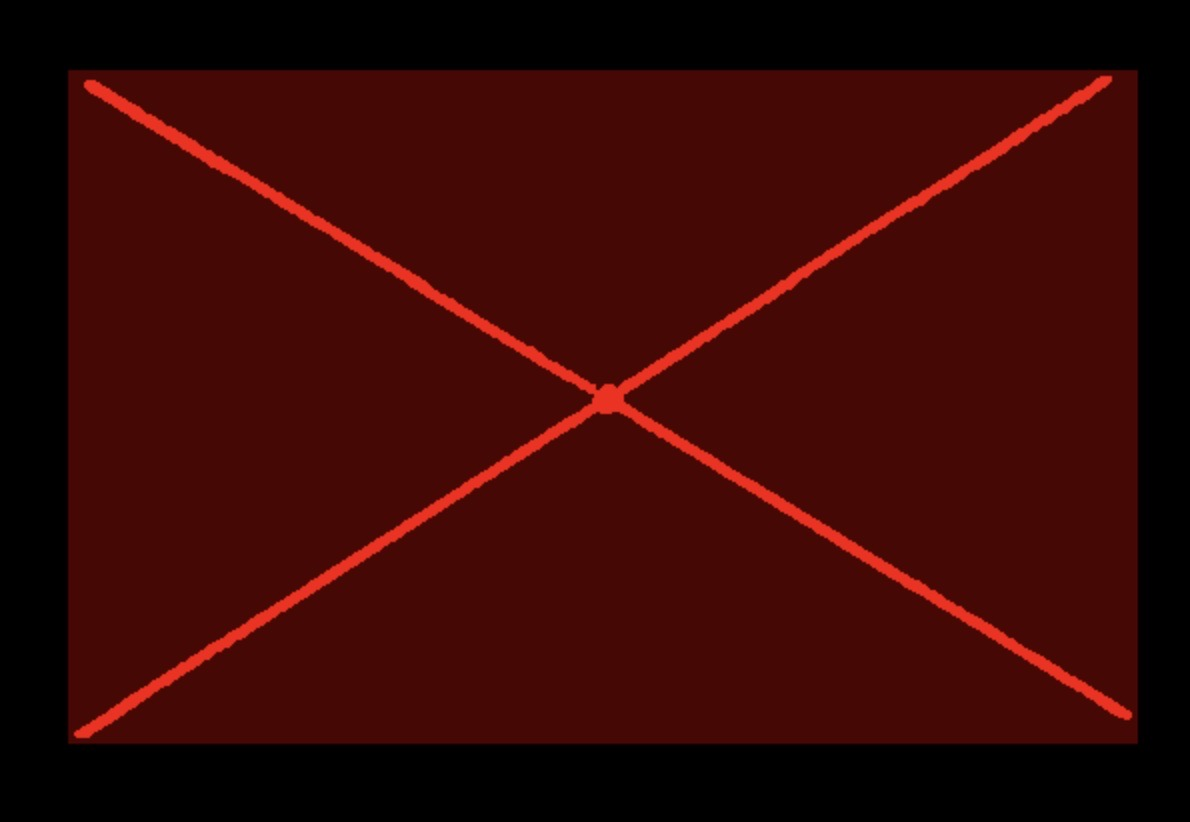
\includegraphics[width=\textwidth]{island}
	\caption{Island met kader gevormd na de floodfill}
	\label{fig:island}
\end{figure}.

\subsection{Bepaling middelpunt}
Om het middelpunt binnen een kader van een island te bepalen wordt de gemiddelde x-- en y--waarde bepaald van alle pixels waarvan de waarde gelijk is aan de island ID plus 2. Pixels die het middelpunt vormen hadden namelijk een lichtblauwe kleur.

\subsection{Find Corners}
Eerst wordt nagegaan of het scherm voornamelijk recht of gekanteld is ten opzichte van de foto. Hiervoor wordt langs de linkerkant van het kader nagegaan hoe hoog de standaarddeviatie van witte pixels is. Indien hieruit blijkt dat het scherm recht ligt, wordt kant per kant afgegaan welke pixels wit zijn en van deze een gemiddelde positie genomen. Indien het scherm gekanteld blijkt te zijn wordt hetzelfde proces herhaald maar dan gebeurt dit diagonaal. De gevonden hoeken zullen zich dan altijd op de rand van het kader bevinden. 

\subsection{Clean Corners}
De vorige methode zal vier hoeken teruggeven. De mogelijkheid bestaat dat wanneer een scherm geroteerd is, twee hoeken rond hetzelfde hoekpunt gevonden worden. Dit geeft eigenlijk geen problemen? Hierdoor is het namelijk duidelijk dat het scherm niet volledig zichtbaar is. Deze methode zal nagaan of twee hoekpunten naar het zelfde punt verwijzen. Indien dit zo is wordt het gemiddelde van de twee opgeslaan als het desbetreffende punt en de andere op "null" geplaats. Daarna moet nog bepaald worden welke de linkse,rechse,onder en boven hoeken zijn. Om deze systematisch bij te houden wordt gebruik gemaakt van een dictionary met als keys "LU","RU","RD"  \space en "LD". Deze toewijzing gebeurt aan de hand van de punten die op ``null `` geplaatst zijn geweest.

\subsection{Reconstructie} \label{reconstructie}
Indien na het controleren van de hoeken nog steeds vier hoeken worden overgehouden, wordt nagekeken of de afstand van overstaande hoeken tot het middelpunt ongeveer gelijk is. Indien dit niet het geval is, dit betekend dat het scherm niet volledig zichtbaar is, maar het kruis toch mooi op de rand van het kader liggen, wordt het punt waarvan de afstand tot het middelpunt het grootst is gepuntspiegeld rond de oorsprong.
In het geval dat er minder dan vier punten gevonden zijn (2 is het minium, zie onze voorwaarden). Wordt gekeken welke hoek null is en wat  de overstaande hoek van deze is zodanig dat, net zoals hiervoor vermeld, deze hoek kan gepuntspiegeld worden. Deze methode is dus ook in staat om te melden wanneer er niet aan de voorwaarden voldaan is geweest. De reconstructie zal volgens de meetkunde slechte resultaten geven wanneer de hoek waaronder de foto getrokken wordt te groot is. Hiervoor is al een oplossing maar deze is nog niet geïmplementeerd (zie secties \ref{Testen} en \ref{Valkuilen} voor meer).

\section{Testen} \label{Testen}
\subsection{Algemeen concept}
De testen maken gebruik van een simpele server waar clients op kunnen verbinden. De client kan vervolgens het absolute tijdverschil meten met een atomische wereldklok.

Eerst en vooral is er een vertraging tussen een aangesloten client en de server, de {\it ping}. Dit is gemeten in milliseconden. De testen meten de vertraging door een bericht met de actuele tijd te verzenden van de server naar de client, en terug. De vertraging is dan de verzonden tijd afgetrokken van de actuele tijd waarmee de ping verkregen is.
In figuur \ref{ping} is de informatieoverdracht zichtbaar. De server berekent de servertijd (TS1) door middel van een API die de exacte wereldtijd teruggeeft, verzonden naar de client en teruggekregen. De uiteindelijke ping is: \[ping = TS2 - TS1\] met TS2 de actuele tijd berekent in de server TS2

\begin{figure}[h]
\centering
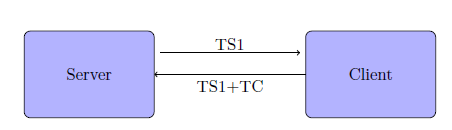
\includegraphics[scale=0.8]{img/img.png}
\caption{Ping} \label{ping}
\end{figure}


Het is niet gegarandeerd dat de klokken van de clients allemaal gesynchroniseerd zijn met de server. Bij het terug verzenden van de client naar de server wordt de clienttijd (TC) bij het bericht gezet.  Met deze TC en de berekende {\it ping} is het mogelijk het tijdsverschil tussen de client en de server te bepalen ($DeltaTime$).
\[DeltaTime = (TC+ping/2) - TS2\]
Deze data wordt vervolgens tussen verschillende browsers en besturingssystemen vergeleken.

\subsection{UDP vs TCP}

UDP heeft in tegenstelling tot TCP geen gevestigde verbinding nodig tussen bijvoorbeeld server en client. TCP zal garanderen dat data correct aankomt door middel van foutopsporing en zal ook in de goede volgorde binnenstromen. Om geen pakketten te verliezen zal TCP deze in een {\it receive buffer} steken en zal de applicatie de ontvangen data pas lezen als ze er klaar voor is. Tegenover UDP waar de data continu zal binnenstromen, ontvangen of niet. Deze zal ook niet aan foutopsporing doen en de juiste volgorde niet gegaranderen. Het is duidelijk dat UDP veel sneller is doordat deze minder stappen en controle bevat. Dit is ook de reden dat het NTP protocol UDP zal gebruiken in plaats van TCP. Het is logisch dat voor een simpele synchronisatie tussen client en server geen complex protocol nodig is. Socket.io gebruikt het TCP protocol in de browser voor veiligheidsredenen.

\subsection{Drift en skew}

Drift zal ervoor zorgen dat een klok niet meer synchroon met zijn oorspronkelijke referentie loopt. Windows lost dit op met een wekelijkse resync (het tijdsverschil zal dus op een sawtooth diagram lijken) terwijl Mac OSX rekening zal houden met de klok skew en andere hardware invloeden om zo beter synchroon te blijven.
Klok skew is het verschil van tijd van een kloksignaal tussen 2 componenten binnen een systeem(zie figuur \ref{skew1} \cite{skew}).

Het tijdsverschil van een windows computer en een atoomklok is gedurende 25 minuten gemeten (zie figuur \ref{drift}). De trendlijn is door de grafiek getrokken en het is duidelijk dat er geen effect ervan te zien is. Over langere tijdsperiode zal de drift groter worden, maar voor de animatie zal dit verwaarloosbaar zijn aangezien het onwaarschijnlijk is dat iemand dagenlang deze zal laten afspelen.

\begin{figure}[H]
\centering
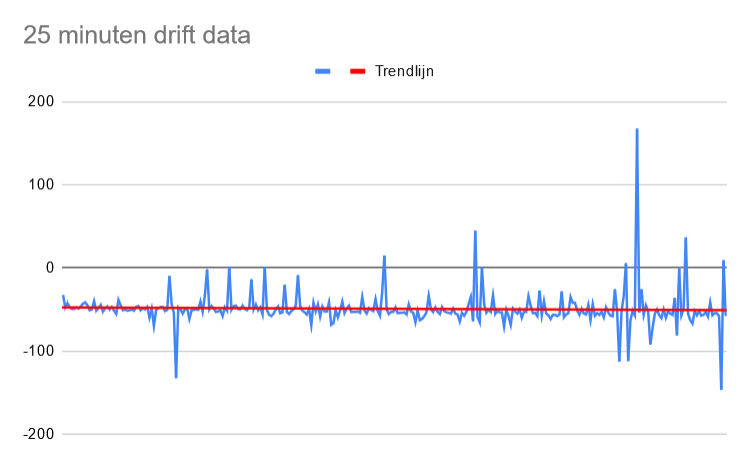
\includegraphics[scale=0.3]{img/drift.png}
\caption{Drift} \label{drift}
\end{figure}

\begin{figure}[H]
\centering
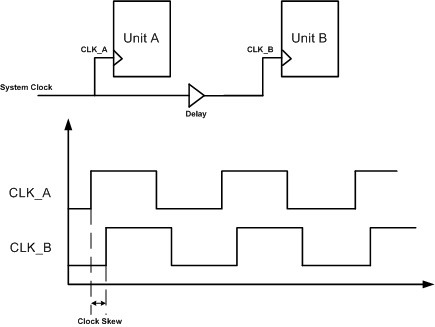
\includegraphics[scale=0.7]{img/skew.jpg}
\caption{Skew} \label{skew1}
\end{figure}


Klok skew kan problemen geven voor correct timings, en zoals eerder vermeld zal OSX dit tegen gaan via software. We zullen niet dieper gaan over de problemen van skew en OSX. 


\subsection{Analyse van de data}
\label{analyse}
Het is duidelijk dat er op elk soort systeem een afwijking gemeten wordt tegenover de referentieklok. Bij sommige operating systems al een groter verschil dan de andere, maar de reden waarom is niet altijd te verklaren of vrijgegeven en zullen hier dus niet verder op in gaan. Elk systeem wordt door het operating system zelf voldoende gesynchroniseerd met een server-klok als referentie en zou in principe maar een paar miliseconden mogen afwijken van deze referentieklok. De fout wordt pas waargenomen in de metingen van het verschil tussen de twee klokken over een netwerk. In deze situatie wordt er een poging gedaan om het verschil tussen device-klok en server-klok te vergelijken door de ping mee in rekening te brengen. De drift van beide klokken gaan over deze tijdsspanne minimaal zijn en gaan geen invloed hebben op deze verschillen. Bij de testen werd ook de gemiddelde ping en standaarduitwijking van de ping per test opgeslagen. Uit deze waarden valt af te leiden dat er bij grote pingfluctuaties ook een grote standaarduitwijking mee gepaard ging en wijst naar inconsistenties binnen het netwerk van ofwel de client ofwel de belasting op de server en is er bijgevolg meer kans op een grotere fout binnen de vergelijking van de klokken. 

\begin{figure}[H]
	\centering
	\begin{subfigure}{.5\textwidth}
		\centering
		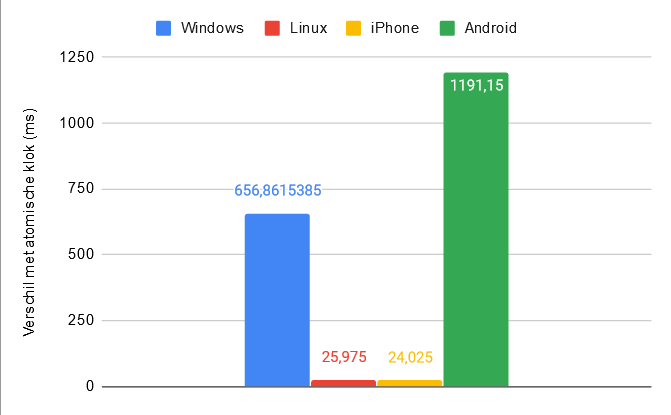
\includegraphics[width=.95\linewidth]{img/mediaan.png}
		\caption{Mediaan van tijdsverschil van elk device.}
		\label{fig:mediaan}
	\end{subfigure}%
	\begin{subfigure}{.5\textwidth}
		\centering
		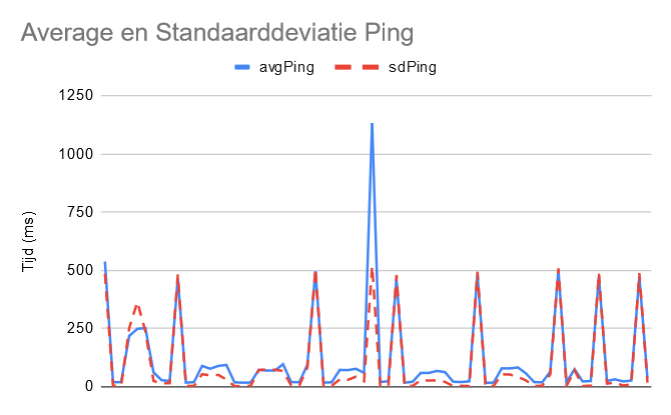
\includegraphics[width=.95\linewidth]{img/ping_results.png}
		\caption{Gemiddelde en standaarduitwijking van de ping met de server. }
		\label{fig:avgPing}
	\end{subfigure}
	\caption{Resultaten van de testen}
	\label{fig:results}
\end{figure}

In figuur \ref{fig:avgPing} is het duidelijk zichtbaar dat er een pieken zijn met hoge standaardafwijkingen. Dit wilt zeggen dat er heel grote fluctuaties zijn in de ping tijdens het synchronisatie proces met 10 opmetingen. Hiermee is de gesynchroniseerde tijd een afwijking hebben met de werkelijke tijd tot ($maxPing - minPing$).






















\section{Valkuilen} \label{Valkuilen}
De grootste valkuil in het detecteren is de reconstructie die nog gevoelig is voor de hoek waaronder de foto genomen is. De meest voor de hand liggende oplossing is werken met een drempel die afhankelijk is van de grootte van het scherm om te kijken wanneer een punt moet gereconstrueerd worden of niet. Deze aanpak lijkt niet ideaal en daarom wordt het volgende voorgesteld. Om later een foto te kunnen weergeven op de schermen moet een transformatiematrix opgesteld worden per scherm. Hieruit kan dan al een transformatiematrix opgesteld worden die de driehoek transformeert naar de originele afmetingen van het scherm. Daarna kunnen de ontbrekende hoekpunten bepaald worden. 